\chapter{実装}\label{cha:Implementation}

本章では、本研究で試作したモータ特性表自動生成ツールの実装について説明する。

\section{特性表生成機能}\label{tokuseihyou_seisei}

% モータ特性表自動生成ツールの処理の流れを図\ref{fig:syori}に示す。\\

% \begin{figure}[t]
% 	\centering
% 	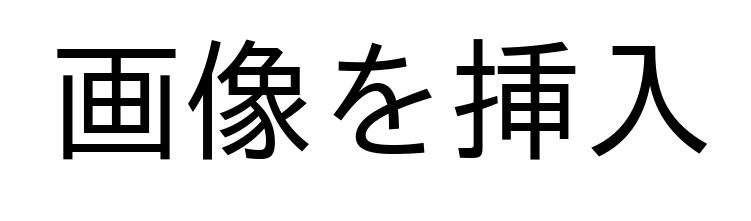
\includegraphics[width=16.5cm,height=10cm]{./Image/sample.png}
% 	\caption{モータ特性表自動生成ツールの処理の流れ}
% 	\label{fig:syori}
%   \end{figure}

特性表生成機能の処理の流れを以下に示す。
\begin{enumerate}
    \item OpenModelicaから出力されたcsvファイルを読み込む
    \item 特性表の各要素を計算するために必要なデータを取得する
    \item 特性表の各要素を計算し求める
    \item 特性表を生成する
\end{enumerate}

以下、各処理について具体的に説明する。

\subsection{csvファイル読み込み}\label{sub:csvfairu}
Pythonで実装するため、Pythonの標準ライブラリのcsvモジュールをインポートし、
csvファイルを読み込む。

\subsection{計算に必要なデータを取得}\label{sub:syutoku_data}
\ref{sub:csvfairu}章で読み込んだcsvファイルから、特性表の各要素を計算するために必要なデータを


\subsection{特性表の各要素を計算}\label{sub:keisan}

\subsection{特性表生成}\label{sub:seisei_hyou}